\chapter{TurtleBot Software}
\label{chap:TurtleBotSoftware}
The TurtleBot Software consists of several launch files which start the processes and load the needed xml descriptions.

\section{Quick Start Guide}
In order to use a laptop to control a TurtleBot several environment variables have to set in the .bashrc, which are show in the following List \ref{chap:ttbsoft:export} for Robot Leonardo.
\begin{itemize}
	\item \verb#export ROBOT=leonardo#
	\item \verb#export TURTLEBOT_3D_SENSOR=kinect#
	\item \verb#export TURTLEBOT_MAP_FILE="$DOMAIN_CONFIG_FOLDER/map_final.yaml"#
	\label{chap:ttbsoft:export}
\end{itemize}
The export \verb#$DOMAIN_CONFIG_FOLDER# should have been set already by the setup script (ttb-setup.sh) found in cnc-turtlebots/configuration/setupscripts.
Otherwise it has to be set to cnc-turtlebots/etc. 
Once these preparations are done the laptop can be used to control it should be placed with closed lid on the layer below the laser scanner. After this is done the USB-hub can be connected with the laptop and the TurtleBot is ready. The setup of the Turtlebot is shown in Figure \ref{fig:ttbback}.
\begin{figure}[htbp]
	\centering
	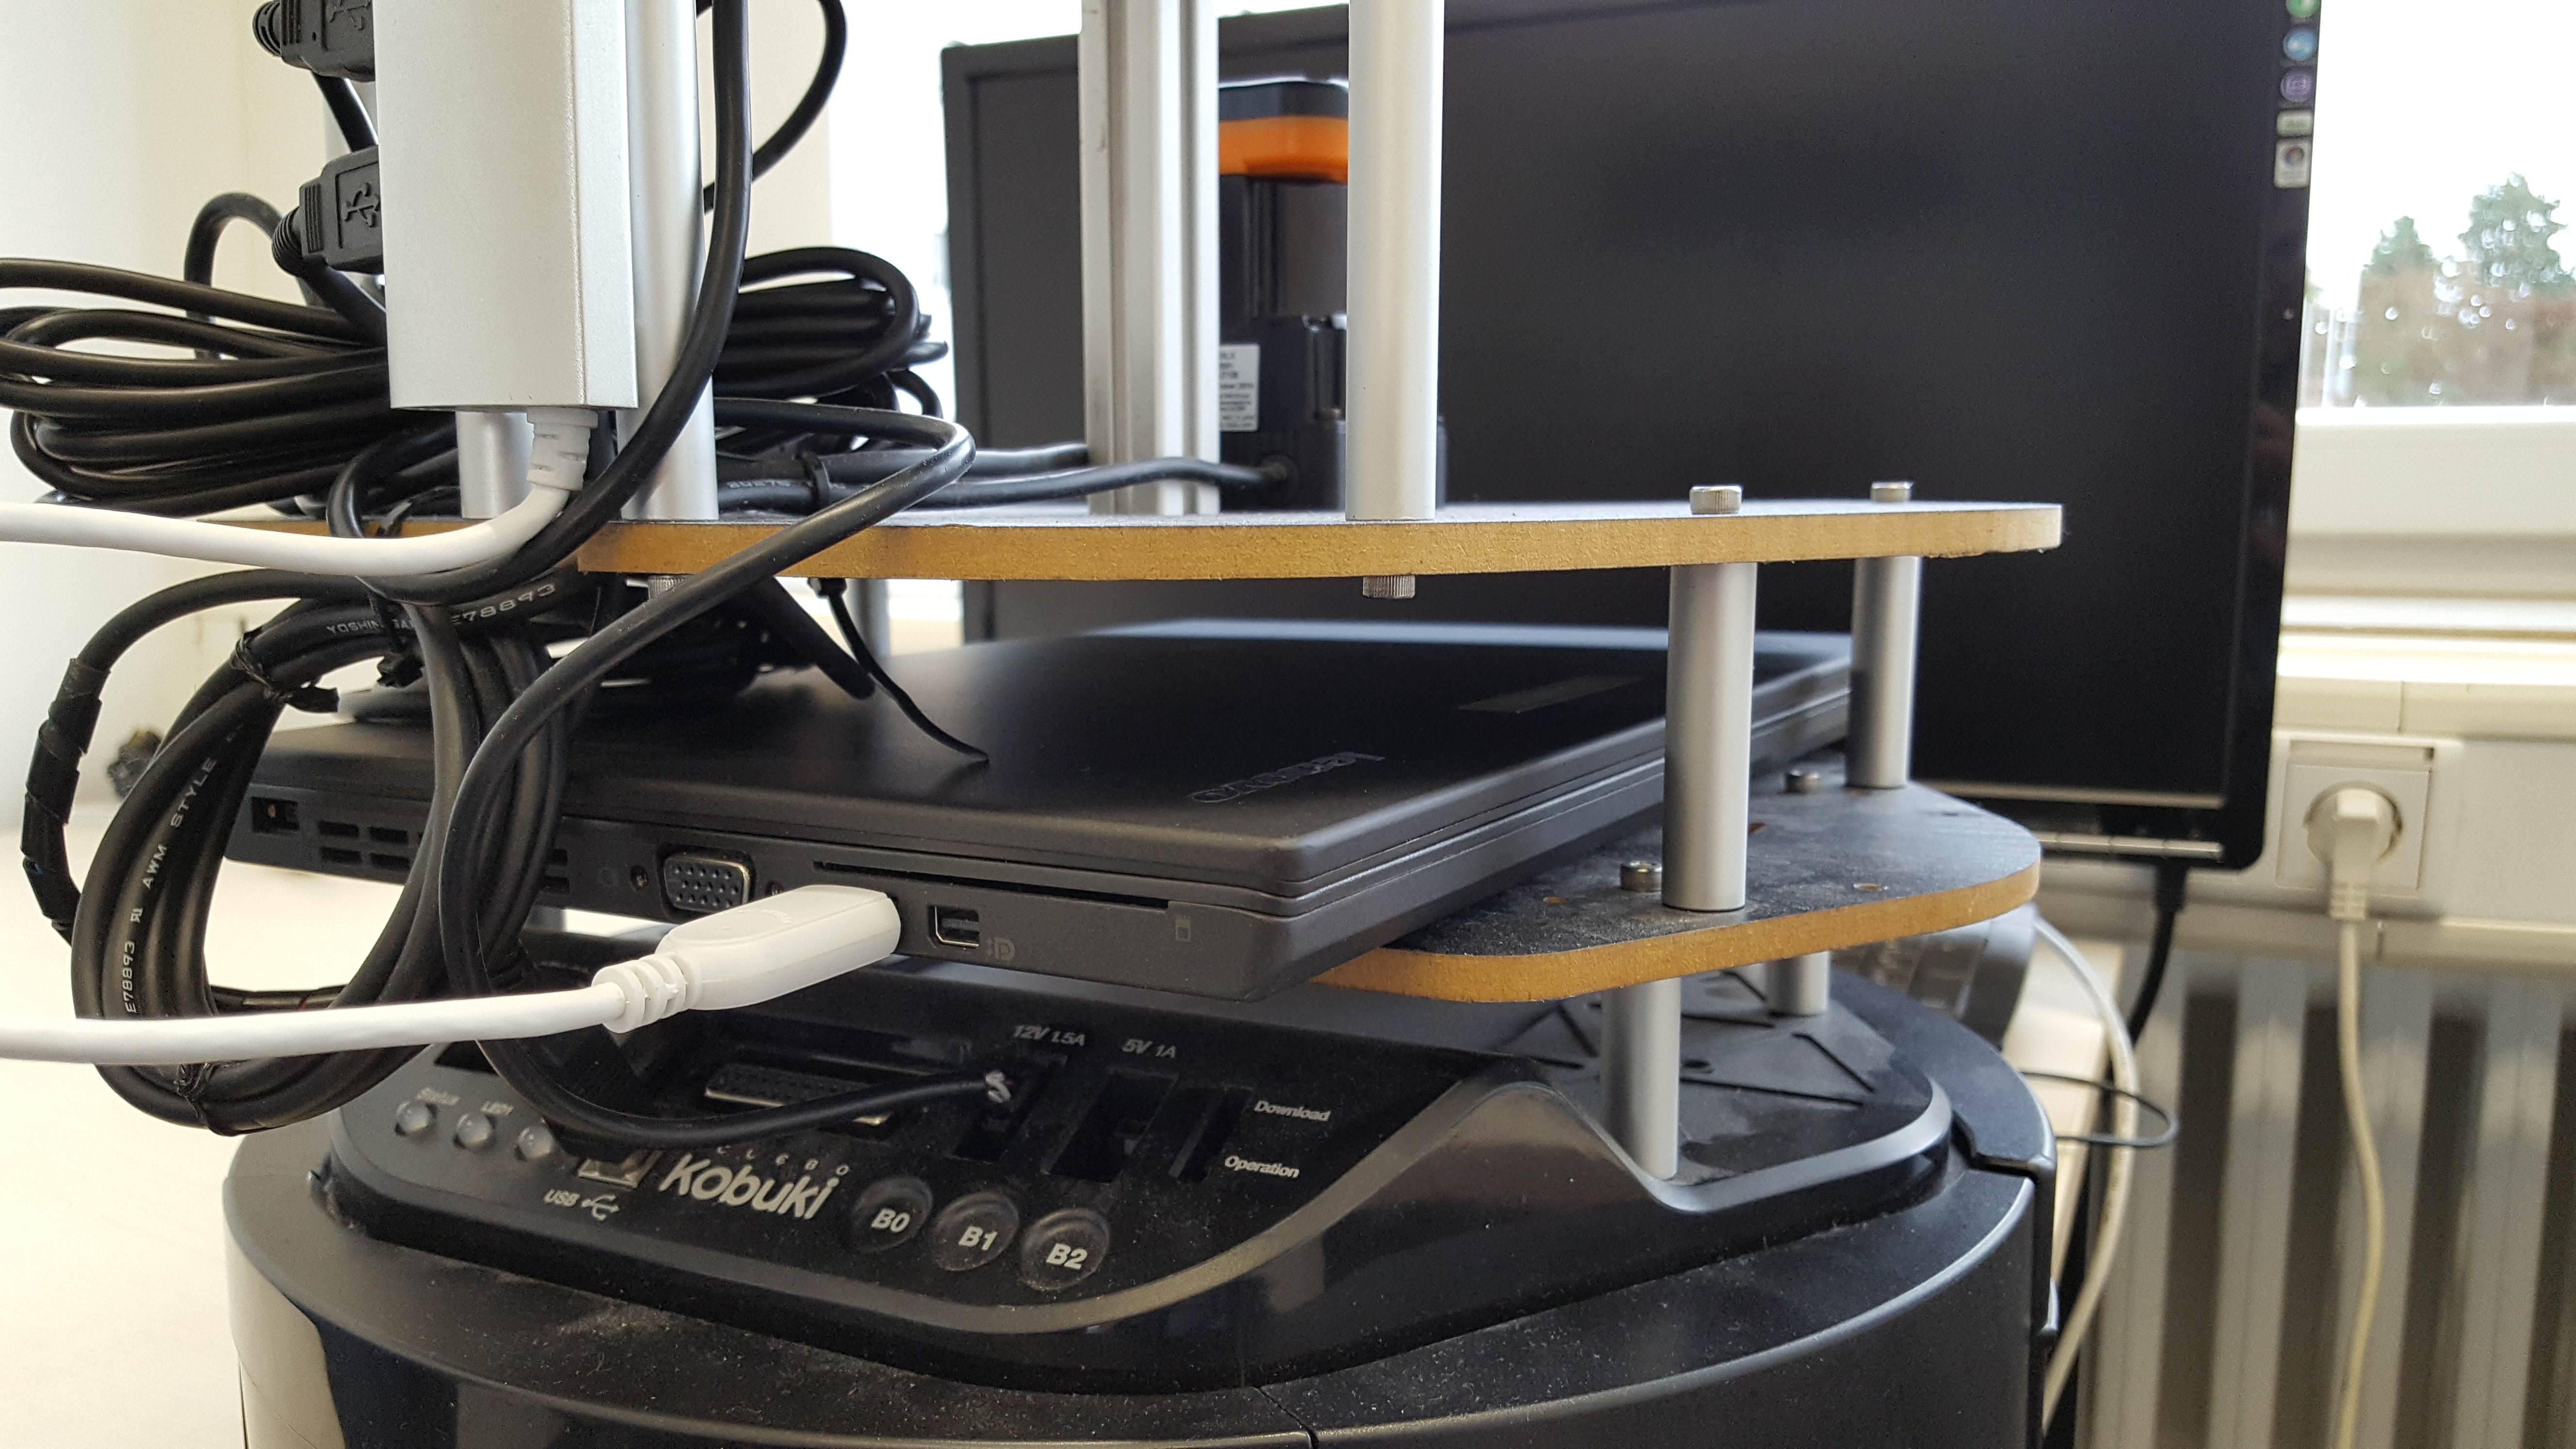
\includegraphics[width=0.6\textwidth]{pic/TurtleBot_back.jpg}
	\caption{TurtleBot setup.}
	\label{fig:ttbback}
\end{figure}
To prepare the laptop/pc to communicate with the TurtleBot these processes are started in three terminals are need on the local laptop/pc in which the following commands have to be executed:
\begin{itemize}
	\item \verb#roscore#
	\item \verb#rosrun ttb_udp_proxy ttb_udp_proxy#
	\item \verb#roslaunch turtlebot_bringup rviz_robot.launch#
\end{itemize}
\verb#rviz_robot.launch# is used to start a GUI that is used to locate the TurtleBot and to create NavGoals which tell the TurtleBot where to drive to. The GUI with buttons for leonardo is depicted in Figure \ref{fig:rviz}. Buttons for additional robots and functions can be added with the plus symbol. the checkbox next to leonardo on the left side of the screenshot has to be clicked to show the model of the robot.
\begin{figure}[htbp]
	\centering
	\includegraphics[width=0.9\textwidth]{pic/rviz.png}
	\caption{Rviz screen.}
	\label{fig:rviz}
\end{figure}
These steps have to be done before starting to processes on the control laptop.
To start the TurtleBot four terminals with a ssh connection to the laptop on the TurtleBot are needed, which can be done either with \verb#ssh tb@robotname.local# or \verb#ssh tb@robotIP#. Once the ssh connections have been established the following commands have to be executed on the terminals:
\begin{itemize}
	\item \verb#roscore#
	\item \verb#rosrun ttb_udp_proxy ttb_udp_proxy#
	\item \verb#roslaunch turtlebot_bringup ninjaturtles.launch#
	\item \verb#roslaunch turtlebot_bringup amcl.launch#
	\end{itemize}
\verb#ninjaturtles.launch# starts all parts of the TurtleBot, \verb#amcl.launch# enables the motion and \verb#ttb_udp_proxy# is used to communicate with other laptops/pcs.
As soon as all processes have been started the TurtleBot's location has to to be set on rviz regarding the position in the real world and its orientation.
This is done by clicking on the pose estimation button with the specific robot name. Afterwards the position and orientation of the TurtleBot can be determined by clicking and holding the left mouse button on the position the TurtleBot should be placed and dragging the cursor in the direction it should face. Once the left mouse button is released position and orientation are determined. To send the TurtleBot to a position the Nav Goal button is used. After clicking this button a position on the map can be marked as a navigation goal in the same way the position of the TurtleBot was determined.   

\section{Drive Topic and Message}
To steer the TurtleBot without using amcl you need to publish a message under a specific topic. A message is published by using \verb#rostopic pub TOPIC MESSAGE#.
The topic used to steer the TurtleBot is named \verb#/cmd_vel_mux/input/teleop# the message is named \verb#geometry_msgs/Twist#. After the command is entered the message contents can be show by pressing tab twice and can be edited before sendin the message with enter. Linear x is used to move the robot forward with a max value of 1.5. Angular z is used to rotate the robot. The max value is 14.
